%!TEX root =  0-main.tex
\section{Background}
\label{sec:background}

%Aiming for a representative study, in our experiments, we adopt Tendermint \cite{buchman2016tendermint}, a blockchain consensus algorithm derived from PBFT \cite{castro1999practical}.   In the following we introduce the system model considered, comment on Tendermint and survey related work.

\subsection{System Model}

We consider a distributed system composed of an unbounded set of client processes that submit transactions (or operations) to a bounded set $\Pi$ of $N$ server processes.   
For simplicity, here we consider that all nodes in $\Pi$ act as \emph{validators} (i.e., nodes that execute the consensus protocol).
The set of nodes is dynamic and known by all nodes.  

Nodes communicate by message passing. 
The system is partially synchronous: it is initially asynchronous when there is no bound on message delays or relative process speeds.
At an unknown moment (i.e., the Global Stabilization Time), the system becomes synchronous, when message delays and processing speed become bounded.

There are up to $F < N/3$ \emph{faulty} or Byzantine nodes; the remaining nodes are \emph{honest}.
Faulty nodes can deviate from their specifications, whereas honest nodes adhere to them.
Cryptographic techniques are used, with adversaries not having (with high probability) the computational power to subvert them.


\subsection{Blockchain Consensus}
\label{tenderback}

We consider permissioned consensus protocols, such as Practical Byzantine Fault Tolerance (PBFT)~\cite{castro1999practical} and Tendermint~\cite{buchman2016tendermint}.
Tendermint consensus operates through three sequential phases, \emph{propose}, \emph{prevote} and \emph{precommit}, which functionally correspond to the \emph{pre-prepare}, \emph{prepare}, and \emph{commit} stages of the PBFT algorithm. The three phases work as follows: 

%\begin{figure}[htbp]
%\centerline{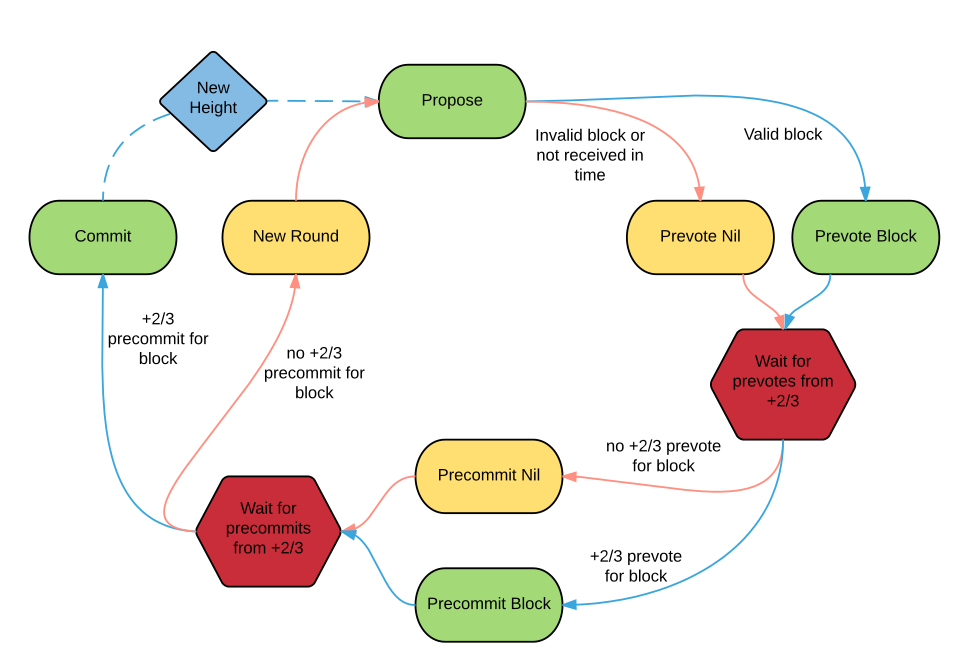
\includegraphics[width=0.8\textwidth]{img/tendermint.png}}
%\caption{Basic Tendermint operation \cite{buchman2016tendermint}}
%\label{Idur}
%\end{figure}


\begin{itemize}
    \item \textbf{Propose}

    The deterministic leader selection function indicates to each node which member of the committee is the current proposer. If a node determines that it is the leader of the current consensus instance it must generate a block, based on its received transactions, and propose it to the network.    Other nodes await the proposal.
    
    \item \textbf{Prevote}

    Once a node receives a proposal it analyzes the block's validity. If the block is valid and was sent from the correct proposer, the node agrees with the proposal and broadcasts a prevote for the block. If the block is invalid, the node prevotes nil. 

    As proposers may not send proposals in a timely manner, due to network issues or Byzantine faults, Tendermint makes use of timeouts. After processing a block, each node awaits a dynamic time interval for the next proposal.  If it is not received within this interval, the node automatically prevotes nil. This timeout is calculated locally according to pre-defined rules, allowing liveness to be maintained as long as the model assumptions hold. 

 After sending its prevote, each node awaits for a quorum. If the node receives a quorum of prevotes for the block, 
 it broadcasts a precommit for the block.   In any other case, including if the node times out when waiting for a quorum, the node 
 broadcasts precommits nil. 
    
    \item \textbf{Precommit}

The precommit phases begins as soon as the node broadcasts a precommit value. If the node receives a quorum of precommits for the block, the block is considered committed and appended to the chain, and consensus for the next block (height) is started.
 Otherwise, if a quorum cannot be reached or if the node timeouts, consensus restarts with the next proposer, in the same height but increasing round. 

\end{itemize}


A primary distinction of Tendermint is the implementation of a rotating proposer mechanism: by using a round-robin approach in which each node proposes only once, the network mitigates censorship \cite{wahrstatter2024blockchain}. % and ensures that an honest proposer eventually assumes leadership. 

Furthermore, unlike PBFT, Tendermint is designed for environments where unknown participants can join. To protect against Sybil attacks\cite{douceur2002sybil}, where a malicious actor might otherwise flood the network with nodes to gain control, the protocol integrates a Proof of Stake (PoS) mechanism. %This economic barrier shifts this is the last candidate.  next esc will revert to uncompleted text. he security assumption from a count of nodes to a distribution of wealth: the system remains secure as long as less than one-third of the total staked tokens are held by Byzantine actors. 
Participants receive rewards for consensus participation, while detected malicious behavior results in the destruction or reduction of their stake via slashing. This design effectively increases the cost of subversion, making it expensive for an adversary to acquire a quorum.

\section{Taxonomy of leader selection strategies}
\label{sec:taxonomy}
%\section{Related Work}

Several works have explored performance-aware leader selection in Byzantine fault-tolerant consensus.
Existing proposals differ substantially in both their objectives and integration strategies. 
To better position our contribution, we classify prior work along seven dimensions (see Table~\ref{related}): 
\textbf{(I) Score Representation}, distinguishing between continuous scores and discrete node classes; 
\textbf{(II) Committee Eviction,} indicating whether nodes may be removed from the active committee; 
\textbf{(III) Evaluation Metrics}, describing the information used to estimate node quality; 
\textbf{(IV) Communication Overhead}, indicating whether the mechanism requires additional protocol messages or coordination phases; 
\textbf{(V) Decoupled Architecture}, capturing whether the optimization is implemented independently from the consensus core and can therefore be reused across different SMR protocols; 
\textbf{(VI) Continuous Evaluation}, indicating whether node quality is continuously updated during execution; and 
\textbf{(VII) Rotation Policy}, describing whether proposer rotation remains active after optimization.

Most related proposals are derived from PBFT-style primary-backup architectures and therefore focus on improving view-change behavior after detecting a slow or faulty leader (e.g., \cite{eischer2018latency, shan2025grouped, zhang2024prestigebft, zhu2025rgpbft}). 
In these systems, node differentiation primarily serves as a ranking mechanism for selecting replacement leaders after a disruption. 
Proposer optimization is often reactive rather than adaptive.

A second recurring characteristic is the reliance on committee eviction to sustain performance (e.g., \cite{du2020performance, huang2023improved, qiao2024enhancing, wen2025mapbft, zhao2022pbft}). 
These approaches remove nodes considered slow, unstable, or suspicious from the active consensus set. 
While effective at increasing throughput in controlled environments, committee reduction introduces a direct trade-off between performance and Byzantine resilience. Removing slow but correct nodes reduces the effective committee size, thereby lowering the maximum number of Byzantine faults the system can tolerate. 
Moreover, modern blockchain deployments already incorporate mechanisms to detect and exclude malicious validators, making additional performance-oriented eviction layers potentially redundant and operationally risky.


%\vspace{-3mm}
\begin{table}[h!]
\centering
\begin{threeparttable}
 \scriptsize 
\newcolumntype{P}[1]{>{\centering\arraybackslash}p{#1}}
\newcolumntype{M}[1]{>{\centering\arraybackslash}m{#1}}
\begin{tabular}
{|M{0.9cm}|M{0.6cm}|M{0.8cm}|M{5cm}|M{1cm}|M{0.8cm}|M{0.8cm}|M{0.8cm}|}
\hline 
\rotatebox{90}{\textbf{Algorithm} } & 
\rotatebox{90}{\shortstack{\textbf{Score}\\\textbf{Type}} } & 
\rotatebox{90}{\shortstack{\textbf{Committee}\\\textbf{Eviction}} } &
\rotatebox{90}{\shortstack{\textbf{Evaluation}\\\textbf{Metrics}} } & 
\rotatebox{90}{\shortstack{\textbf{Communic.}\\\textbf{Overhead}} } &
\rotatebox{90}{\shortstack{\textbf{Decoupled}\\\textbf{Architecture}}  } & 
\rotatebox{90}{\shortstack{\textbf{Continuous}\\\textbf{Evaluation}} } & 
\rotatebox{90}{\shortstack{\textbf{Rotation}\\\textbf{Policy}} }\\ 
\hline
\cite{du2020performance} &
C&
Y &
Consensus participation and proposal success ratio &
Y &
Y &
Y &
N\\
\hline

\cite{eischer2018latency} &
C&
N&
Per-node consensus latency measured through active probing by clients&
Y\tablefootnote{Multiple consensus.}&
Y &
N &
N \\
\hline

\cite{huang2023improved} &
D&
Y &
Composite reputation derived from performance and participation &
Y &
N &
Y &
N\\
\hline

\cite{qiao2024enhancing} &
D&
Y &
Latency, availability, activity level, and consensus contribution &
Y &
N &
Y &
N\\
\hline

\cite{shan2025grouped} &
D&
N &
Behavioral classification and response-time analysis &
Y &
N &
Y &
N\\
\hline

\cite{wen2025mapbft} &
C&
Y &
Latency measurements combined with reputation signals &
Y &
N &
Y &
N\tablefootnote{The primary is the node with the most voting power \cite{wen2025mapbft}. If voting power changes, a new node can become the primary even without suspected failure. However, the algorithm does not perform intentional leader rotation.}\\

\hline
\cite{yu2024adaptive} &
C&
N &
Observed leader throughput during evaluation windows &
N &
Y &
N &
N\\
\hline

\cite{zhang2024prestigebft} &
C&
N&
Historical leader success, measured by committed blocks&
Y&
Y\tablefootnote{For systems without leader rotation.} &
Y &
N \\
\hline

\cite{zhao2022pbft} &
D&
Y &
Binary success/failure outcomes of consensus participation &
N &
N &
Y &
N\\
\hline

\cite{zhu2025rgpbft} &
C&
N &
Consensus participation consistency, and failure frequency &
Y &
N &
Y &
N\\
\hline

This paper &
C&
N &
Consensus duration&
Y &
Y &
Y &
P\\
\hline

\end{tabular}
\caption{Taxonomy of leader selection strategies.}
\begin{tablenotes}
\small
\item Legend: Continuous (C) scores allow fine-grained proposer differentiation, while Discrete (D) scores classify nodes into categories. Committee Eviction indicates whether nodes may be removed from the active consensus committee. Proportional (P) rotation biases proposer frequency according to performance, whereas No rotation (N) maintains the primary/proposer until a view change is proposed.
\end{tablenotes}
\label{related}

\end{threeparttable}
\end{table} 

The surveyed literature also differs in how it treats proposer fairness. 
Many PBFT-derived optimizations effectively converge toward fixed or weakly rotating leaders, increasing susceptibility to censorship and centralization. 
%Yu et al. \cite{yu2024adaptive} partially address this issue by enforcing equal rotation among nodes above a performance threshold. 
Our approach instead adopts proportional prioritization: higher-performing nodes are selected more frequently, while all nodes remain eligible proposers. This preserves continuous rotation while still exploiting topology-aware performance asymmetries.
%[OUR APPROACH CAN, DEPENDING ON THE CONFIGURED VALUES (E.G. ALLOWING SCORE TO BE UP TO +-100\% OF STAKE), REMOVE NODES FROM ROTATION (BUT KEEP THEM IN THE COMMITTEE). THIS IS INTENTIONAL AND ALLOWS FOR MAXIMUM THROUGHPUT AT THE COST OF CENSORSHIP RESILIENCE]

Finally, existing work generally treats proposer performance as an abstract property associated with computational speed or node responsiveness, with limited investigation into how network topology shapes consensus execution. 
Our experiments show that proposer placement directly affects overall consensus latency, influencing the duration of subsequent protocol phases. 
In geo-distributed deployments, proposer location therefore becomes a first-order determinant of consensus efficiency rather than merely a secondary implementation detail.

Table~\ref{related} highlights two dominant trends in prior work: (i) performance optimization through committee reduction, and (ii) tightly coupled protocol-specific leader management. 
Our approach differs in that it preserves the full committee and the original Byzantine threshold while continuously adapting proposer frequency based on observed consensus performance. 
Unlike eviction-based strategies, proposer prioritization improves throughput without sacrificing resilience or requiring invasive protocol modifications.



%This reliance on PBFT also creates an evaluation gap in the literature. 
%%Existing comparisons frequently focus on legacy PBFT baselines under heavy Byzantine attacks. Consequently, 
%It remains unclear how modern production-grade SMR systems with native Byzantine removal (such as Tendermint or HotStuff) would benefit from these proposed optimizations.
%%
%Additionally, while these primary-replica systems inherit a susceptibility to censorship, the surveyed literature largely leaves this vulnerability unaddressed. A notable exception is the work by Yu et al. \cite{yu2024adaptive}, which mitigates censorship by enforcing a uniform rotation among all nodes that exceed a baseline performance threshold. 
%
%In contrast, our approach balances performance and censorship resistance by biasing the leader rotation toward high-performing nodes. This design enhances throughput while preserving continuous rotation across the committee. Tailored specifically for modern SMR architectures, our solution maintains original Byzantine fault-tolerance bounds and acts as a non-invasive plugin that optimizes proposer selection without modifying the underlying consensus algorithm.
%
%Finally, a recurring limitation across prior work is the superficial treatment of consensus latency. The assumption that computationally weak or topologically distant nodes degrade performance is often accepted without empirical investigation. Our experiments challenge this oversimplification, demonstrating that node-to-node network latency is a critical factor that dictates not only individual step durations, but also the dynamic composition of the quorums that actively drive consensus.
